\documentclass[11pt, letterpaper]{article}
\usepackage[margin=1in]{geometry}
% \usepackage[top=1in, bottom=1in, left=0.75in, right=0.75in, paperwidth=8.5in, paperheight=11in]{geometry}
\usepackage{amsfonts, amssymb, amsmath}
\usepackage{tikz, pgfplots}
\usepackage{graphicx} % insert image files
\usepackage{float} % [H] to put images 'HERE'

\title{\LaTeX\ Tutorial 6: Packages, Macros, and Graphics}
\author{Joel M. Brigida: ADolbyB}
\date{} % leave blank for no date or \today for current date.

\def\eq1{y=\dfrac{x}{3x^2+x+1}} % Custom macro command (Can add $ $ but not advised.)
\newcommand{\set}[1]{\setlength\itemsep{#1em}} % Custom Command for increasing line separation

\newcommand\calculator{\tikz{ % custom calculator icon
    \node (c) [inner sep=0pt, draw, fill=black, anchor=south west]{\phantom{N}};
    \begin{scope}[x=(c.south east), y=(c.north west)]
    \fill[white] (0.1, 0.7) rectangle (0.9, 0.9);
    \foreach \x in {0.1, 0.33, 0.55, 0.79}{
    \foreach \y in {0.1, 0.24, 0.38, 0.53}{
    \fill[white] (\x, \y) rectangle +(0.11, 0.07);}}
    \end{scope} }}
    \def\calcicon#1{\noindent#1 \calculator}

\pgfplotsset{compat=1.18} % fix pgfplots compatibility error
\begin{document}
\maketitle
\thispagestyle{empty} % Remove Title Page Number

\pagebreak
\setcounter{page}{1} % Make Page #1 after the title page.

\begin{center}
    \textbf{Critical Thinking Questions}
\end{center}

\begin{figure}[H] % Place image HERE. Also valid: [t] = TOP, [b] = BOTTOM. Note: [H] requires float pkg
    \centering % center the image and scale to 40% of the text width:
    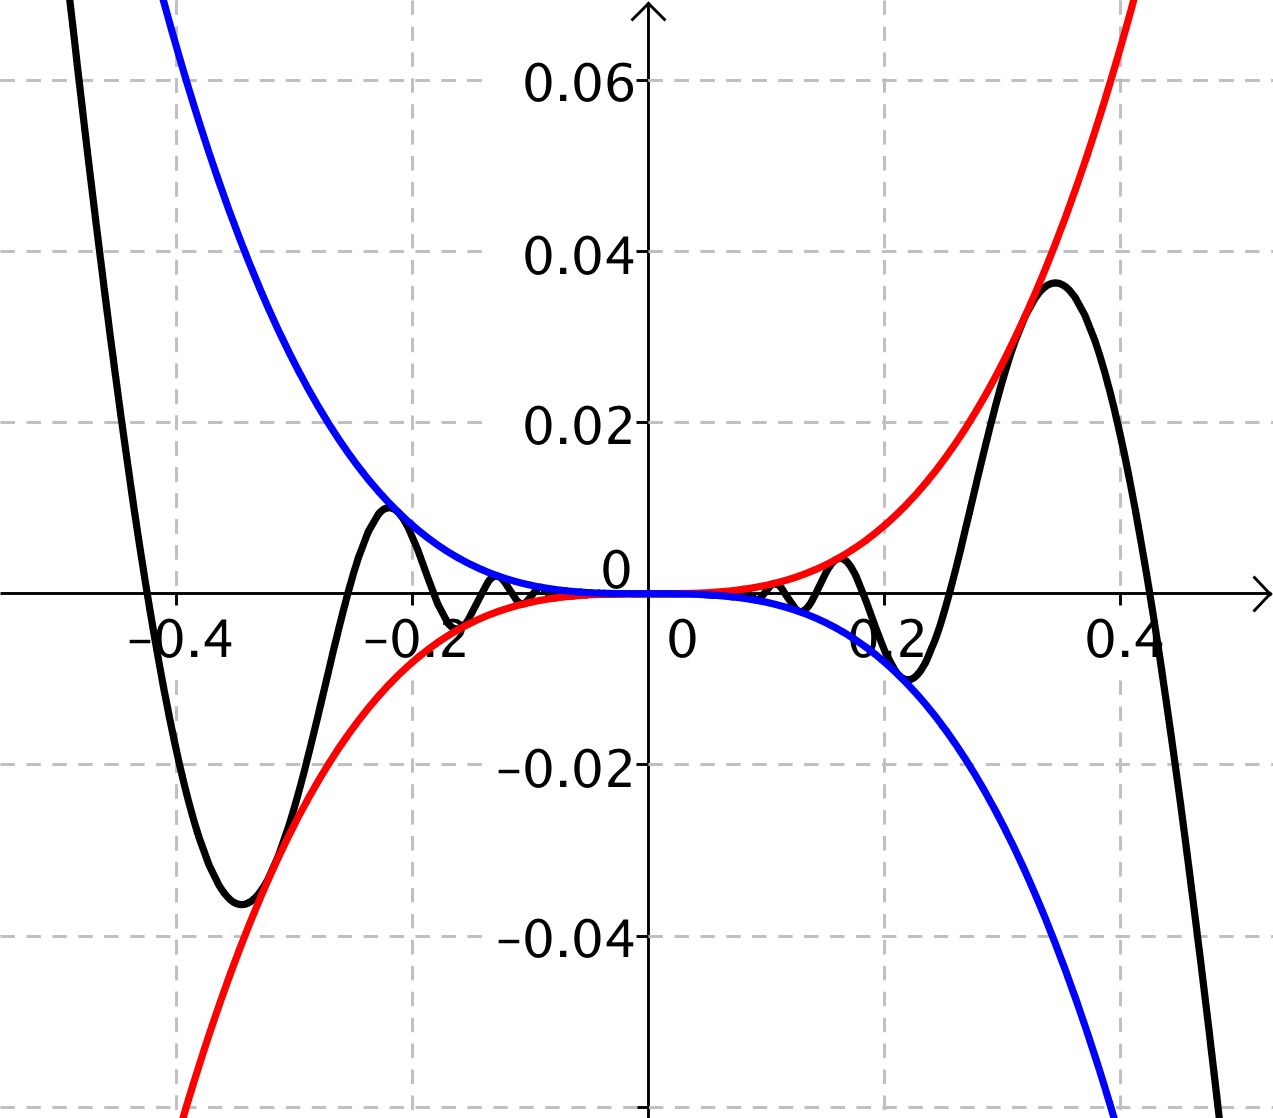
\includegraphics[width=0.4\textwidth]{limit.png} % also valid: [scale=x.x], [height=X.Xin], [width=X.Xin]
    \caption{The Squeeze Theorem} % Place caption BELOW image.
\end{figure}

\begin{enumerate}
    \set{1.2} % Calling custom command for line separation.
    \item \calculator\ Let's examine the function $\eq1$. % calling macro inside document.
    \item This is the symbol for the set of all real numbers: $\mathbb{R}$ % uses amsfonts pkg
    \item This is the symbol for the set of all integers: $\mathbb{Z}$
    \item This is the symbol for the set of all rational numbers: $\mathbb{Q}$
    \item Is it possible for a sequence to converge to two different numbers? If so, give an example. If not,
        explain why not.
    \item Explain how to use partial sums to determin if a series converges or diverges. Give an example.
    \item Explain Why $ \int\limits_{1}^{\infty} f(x)\, dx$ and $ \sum\limits_{n=1}^{\infty} a_n $ need not 
        converge to the same value, evenif they are both convergent.
    \item In your own words, explain the Alternating Series Remainder Theorem. How is this theory 
        useful?
    \item Explain the difference between absolute and conditional convergence.\\
        Give an example of each.
    \item The ratio test is inconclusive if $ \displaystyle{\lim\limits_{n \to \infty} \left| 
        \frac{a_{n+1}}{a_n} \right| = 1} $. Give an example of one convergent and divergent series for which
        $ \displaystyle{\lim\limits_{n \to \infty} \left| \frac{a_{n+1}}{a_n} \right| = 1} $. Explain how you 
        determined your examples.
\end{enumerate}


\end{document}